\documentclass[tikz,border=10pt]{standalone}
\usetikzlibrary{shapes.geometric,backgrounds,calc,positioning,decorations.pathreplacing}

\makeatletter
\tikzset{
    block filldraw/.style={% only the fill and draw styles
        fill=#1!30},
    block rect/.style={% fill, draw + rectangle (without measurements)
        block filldraw, rectangle},
    block/.style={% fill, draw, rectangle + minimum measurements
        block rect, minimum height=0.6cm, minimum width=0.0001cm},
    from/.style args={#1 to #2}{% without transformations
        above right={0cm of #1},% needs positioning library
        /utils/exec=\pgfpointdiff
            {\tikz@scan@one@point\pgfutil@firstofone(#1)\relax}
            {\tikz@scan@one@point\pgfutil@firstofone(#2)\relax},
        minimum width/.expanded=\the\pgf@x,
        minimum height/.expanded=\the\pgf@y}}
\makeatother
  
\begin{document}
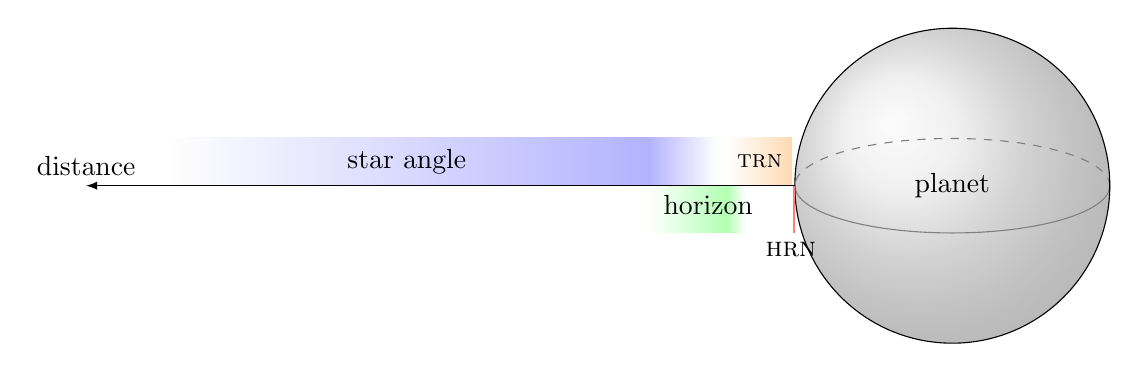
\begin{tikzpicture}[>=latex]
\node[above] at (-11,0) (distance) { distance };
\node[block filldraw = orange, from={-2.87,0 to -2.04,0.6}, shading = axis, left color=white, right color=orange!30] {\small\textsc{trn}};
\node[block filldraw = green, from={-2.87,-0.6 to -2.7,0.0}, shading = axis, left color=green!30, right color=white] { };
\node[block filldraw = green, from={-3.87,-0.6 to -2.87,0.0}, shading = axis, left color=white, right color=green!30, align=right] { };
\node[below] at (-3.1, 0.0) { horizon };
\node[block filldraw = blue, from={-3.87,0 to -3.0,0.6}, shading = axis, left color=blue!30, right color=white] { };
\node[block filldraw = blue, from={-10,0 to -3.87,0.6}, shading = axis, left color=white, right color=blue!30] { star angle};
%\node[block filldraw = red, from={-2.1,-0.6 to -2.0,0}, shading = axis, left color=red!30, right color=white] (hrn){ };
\shade[ball color=gray!40, opacity=0.4] (0,0) circle (2cm);
\draw[color=gray] (-2,0) arc (180:360:2 and 0.6);
\draw[dashed,color=gray] (2,0) arc (0:180:2 and 0.6);
\draw (0,0) circle (2cm);
\node (0,0) (planet) { planet };
\node[below] at (-2.05,-0.6) {\textsc{hrn}};
\draw[->]  (-2,0) -- (-11,0);
\draw[color=red!50]  (-2.01,-0.6) -- (-2.01,0.0);
\end{tikzpicture}
\end{document}
